\section{Experimental Evaluation}\label{sec:eval}

\subsection{Datasets}


Table~\ref{table:datasets}, shows the summary of the dataset we use for our evaluation. We evaluate our models on three datasets provided by \cite{tvkasteren2010}, each home having sensors deployed. Figure~\ref{fig:houses} displays the floor plans and sensor locations of the three residences. Each home is a singe occupant home, so there is no concurrent conflicting activities. The activities are documented manually using bluetooth/diary by the occupant, and is used as 'ground truth' data. The data is collected for a period of almost 24 days with at least 2000 sensor events and 245 activity instances.

\begin{figure}
	\centering
	\begin{subfigure}[b]{0.25\textwidth}
		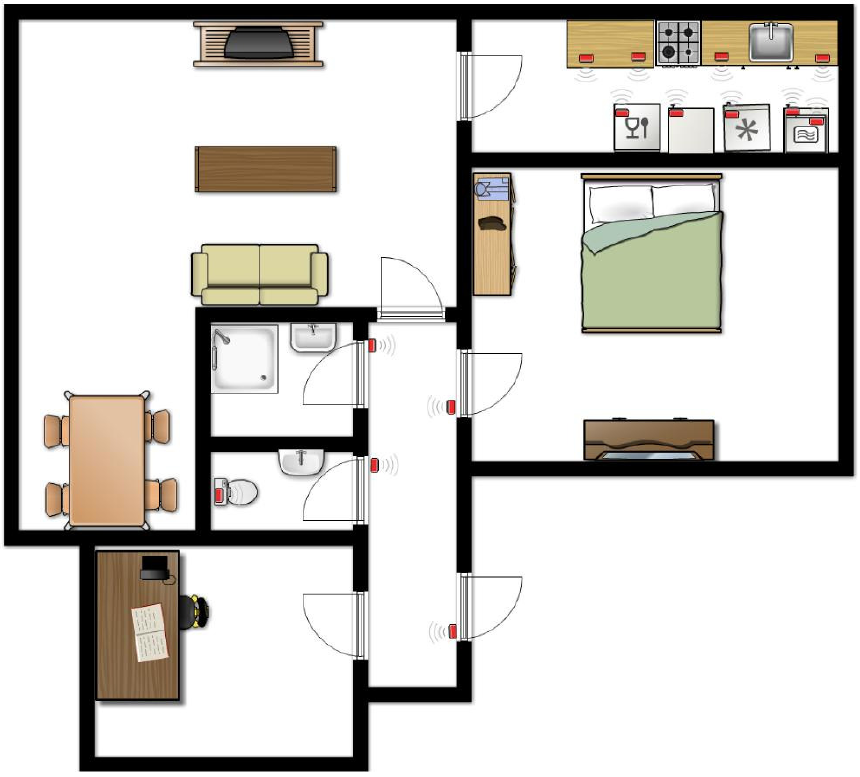
\includegraphics[width=\textwidth]{fig/houseA.png}
		\caption{House A}
		\label{fig:houseA}
	\end{subfigure}
	~
	\begin{subfigure}[b]{0.25\textwidth}
		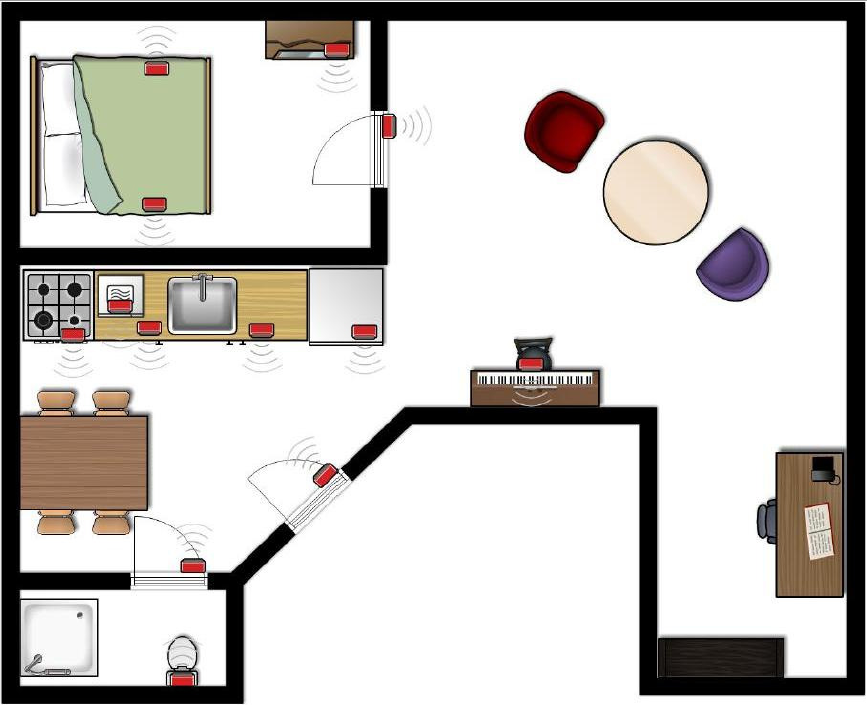
\includegraphics[width=\textwidth]{fig/houseB.png}
		\caption{House B}
		\label{fig:houseB}
	\end{subfigure}
	\\
	\begin{subfigure}[b]{0.25\textwidth}
		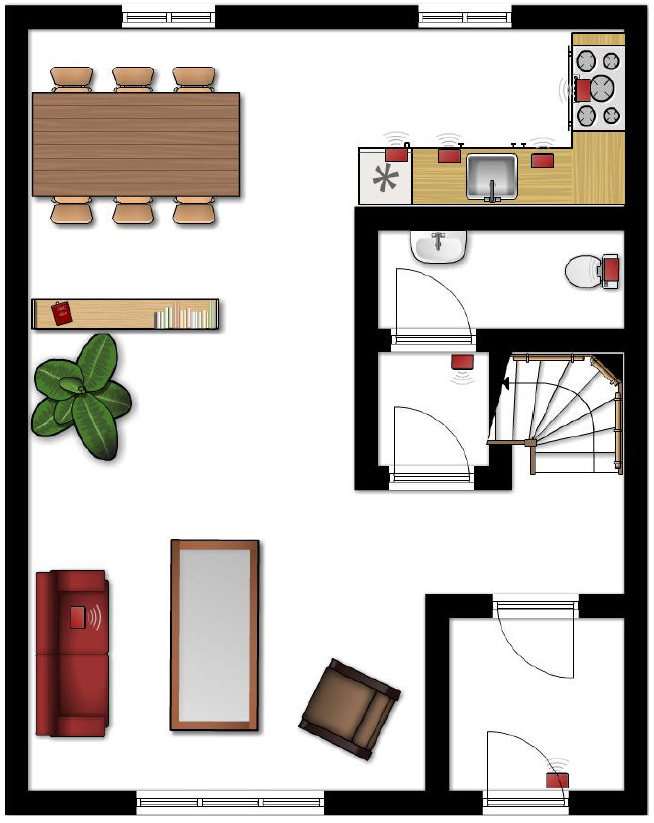
\includegraphics[height=\textwidth,angle=90]{fig/houseC1.png}
		\caption{House C first floor}
		\label{fig:houseC1}
	\end{subfigure}
	~
	\begin{subfigure}[b]{0.25\textwidth}
		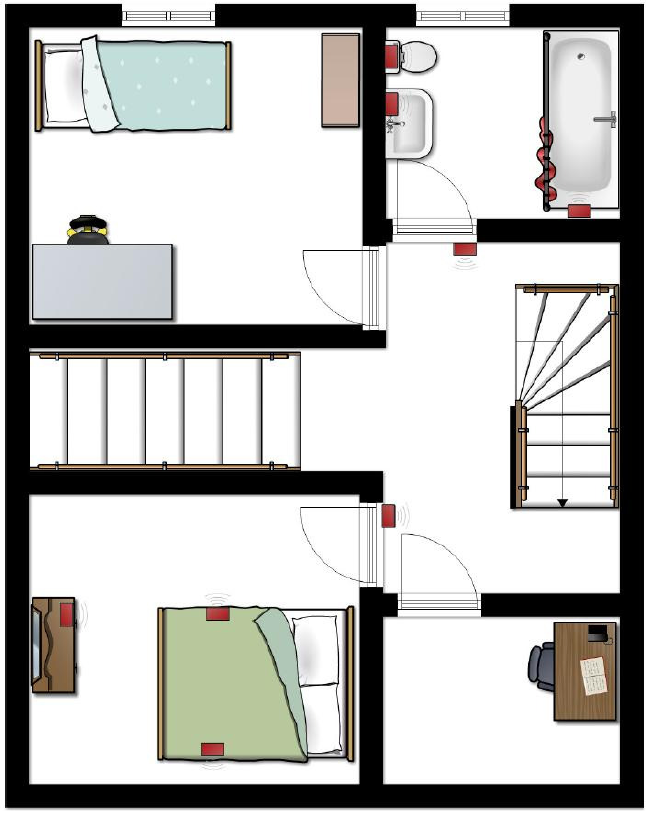
\includegraphics[height=\textwidth,angle=90]{fig/houseC2.png}
		\caption{House C second floor}
		\label{fig:houseC2}
	\end{subfigure}
	\caption{Home floor plans and sensor locations.}\label{fig:houses}
\end{figure}


%The Kasteren dataset is recording a 26-year-old man. He lives alone in a three-room apartment where 14 state-change sensors were installed. Locations of sensors include doors, cup- boards, refrigerator and a toilet flush sensor. Sensors were left unattended, collecting data for 28 days in the apartment. This resulted in 2120 sensor events and 245 activity instances.


%The Kasteren dataset is recording a 26-year-old man. He lives alone in a three-room apartment where 14 state-change sensors were installed. Locations of sensors include doors, cup- boards, refrigerator and a toilet flush sensor. Sensors were left unattended, collecting data for 28 days in the apartment. This resulted in 2120 sensor events and 245 activity instances.
%
%As shown in the table, for Kasteren dataset we have three houses with 14, 23, 21 sensors, respectively.

%The tableis an example of referenced \LaTeX elements.
 
\begin{table*}[t!]
\small
\begin{center}
\begin{tabular}{|c|c|c|c|}
\hline
\textbf{Type} & \emph{House A} & \emph{House B} & \emph{House C}\\ \hline
\textbf{Age} & 26 & 28 & 27\\ \hline
\textbf{Gender} & M & M & M\\ \hline
\textbf{Setting} & Apartment & Apartment & House\\ \hline
\textbf{Room} & 3 & 2 & 6\\ \hline
\textbf{Duration(days)} & 25 & 14 & 19\\ \hline
\textbf{Sensors} & 14 & 23 & 21\\ \hline
\textbf{Activities} & 10 & 13 & 16\\ \hline
\textbf{Annotation} & Bluetooth & Diary & Bluetooth\\ \hline
\end{tabular}
\end{center}
%\vspace{-0.1cm}
\caption{Dataset description}
\label{table:datasets}
\vspace{-0.3cm}
\end{table*}




%\subsection{Comparative Analysis Metrics}
%
%\begin{equation}
%Precision = \frac{TP}{TP+FP}
%\end{equation}
%
%\begin{equation}
%Recall = \frac{TP}{TP+FN}
%\end{equation}
%
%\begin{equation}
%Accuracy = \frac{TP+TN}{TP+TN+FP+FN}
%\end{equation}
%
%\begin{equation}
%F-Measure = \frac{2\cdot Precision\cdot Recall}{Precison+Recall}
%\end{equation}

%The Matthews correlation coefficient is used in machine learning as a measure of the quality of binary (two-class) classifications, introduced by biochemist Brian W. Matthews in 1975. It takes into account true and false positives and negatives and is generally regarded as a balanced measure which can be used even if the classes are of very different sizes. The MCC is in essence a correlation coefficient between the observed and predicted binary classifications; it returns a value between ‚àí1 and +1. A coefficient of +1 represents a perfect prediction, 0 no better than random prediction and ‚àí1 indicates total disagreement between prediction and observation.

%\begin{equation}
%MCC=\frac{TP\cdot TN-FP\cdot FN}{\sqrt{(TP+FP)\cdot (TP+FN)\cdot (TN+FP)\cdot (TN+FN)}}
%\end{equation}


\subsection{Discussion}

\begin{figure}
	\centering
	\begin{subfigure}[b]{0.4\textwidth}
		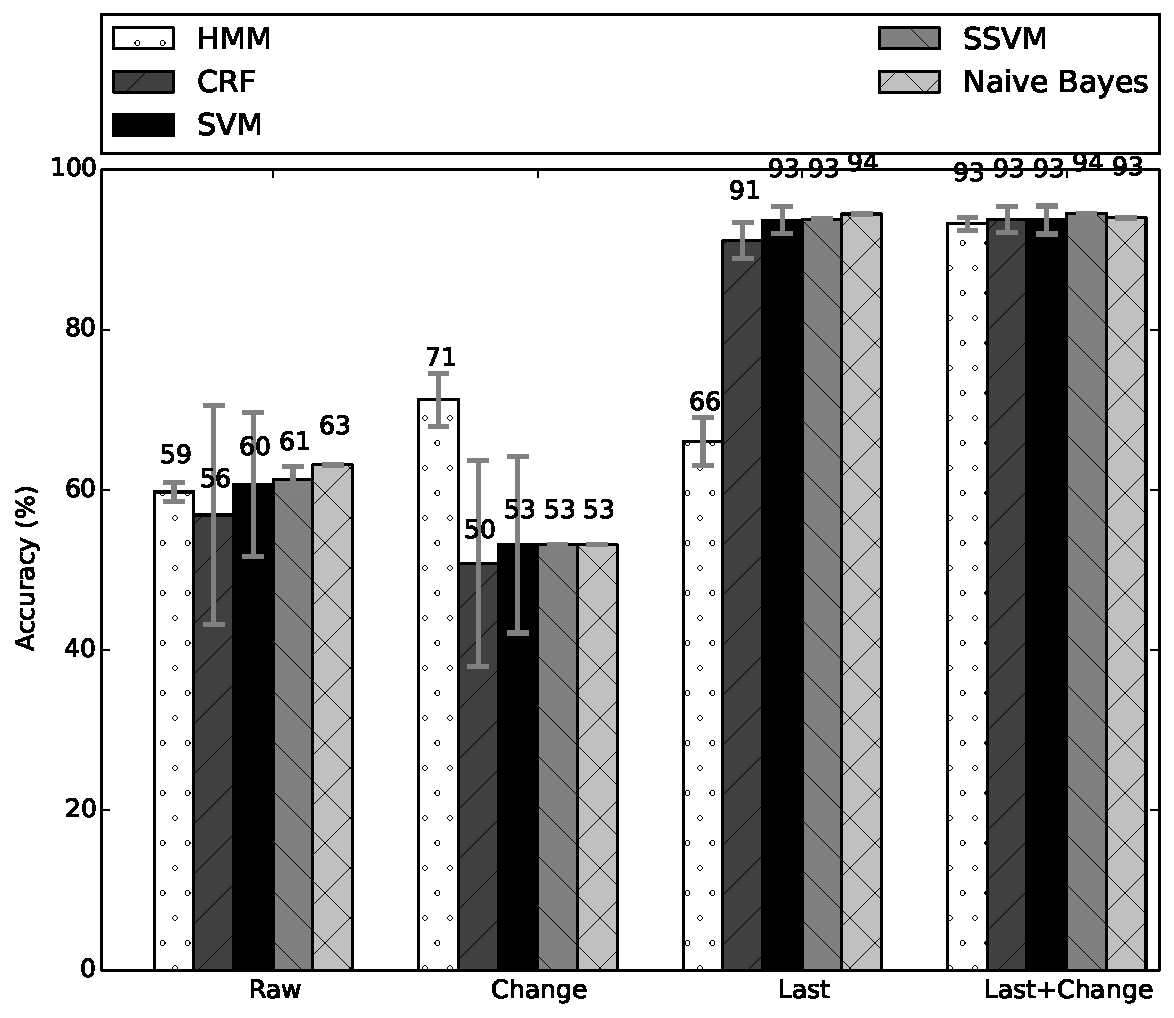
\includegraphics[height=\textwidth]{../../src/reports/A.pdf}
		\caption{House A}
		\label{fig:chouseA}
	\end{subfigure}
	~~\hspace{1in}
	\begin{subfigure}[b]{0.4\textwidth}
		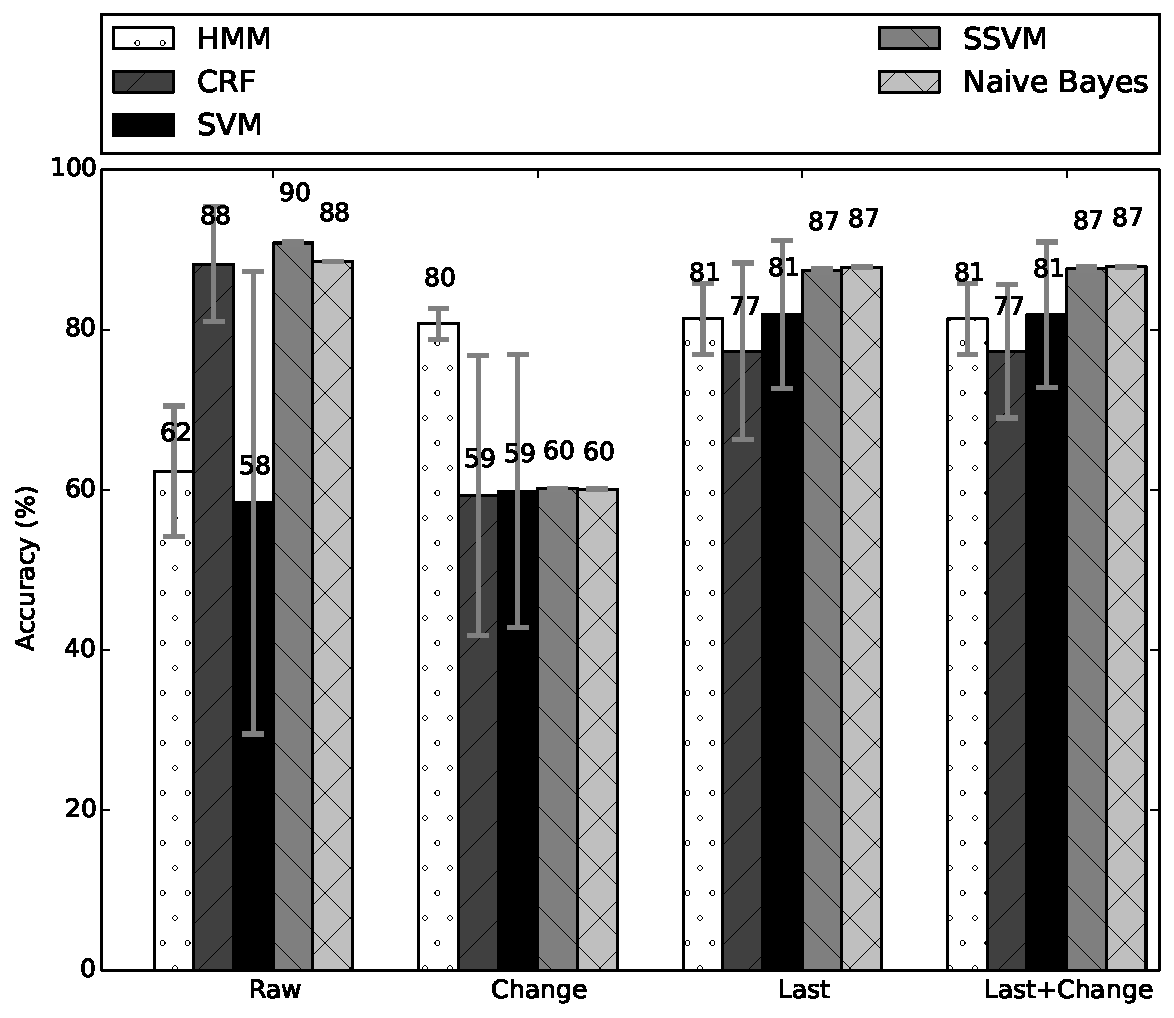
\includegraphics[height=\textwidth]{../../src/reports/B.pdf}
		\caption{House B}
		\label{fig:chouseB}
	\end{subfigure}
	
	\begin{subfigure}[b]{0.4\textwidth}
		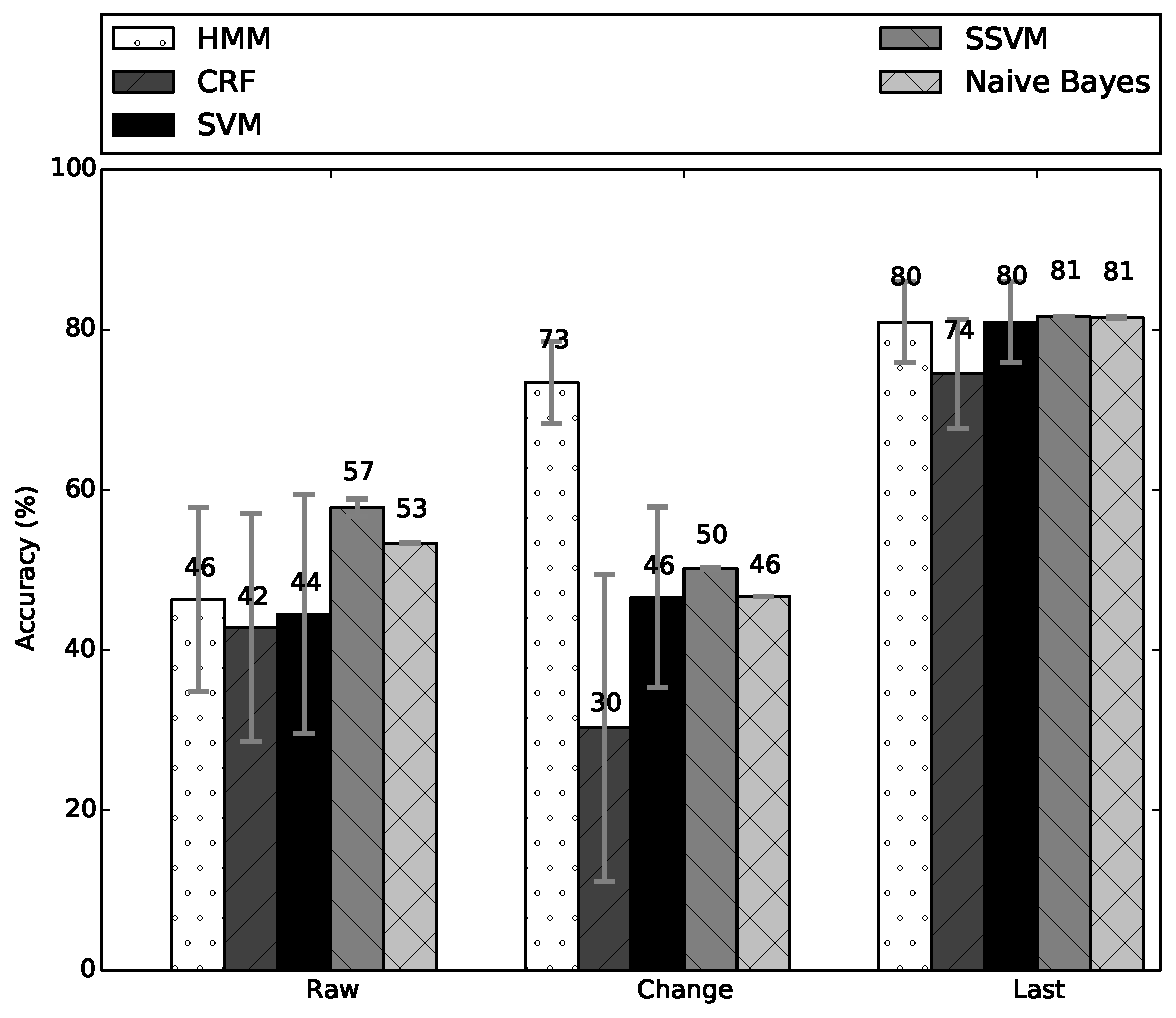
\includegraphics[height=\textwidth]{../../src/reports/C.pdf}
		\caption{House C}
		\label{fig:chouseC}
	\end{subfigure}
	\caption{Method comparison for the houses.}\label{fig:comparison}
\end{figure}


We use 5-fold cross validation to evaluate different methods. We use the timeslice duration of 1 sec for all our evaluation. 
Figure~\ref{fig:comparison}, compares the accuracy of the different models. 
We observe that the \emph{last} and \emph{last+change} feature representations have the highest accuracy compared to \emph{raw} and \emph{change} in House A and House C. We note that combining \emph{last} and \emph{change} feature set  has similar or better accuracy compared to other feature representations. However, in House B the \emph{raw} representations performs better using SSVM.
We believe that the amount of training data available for House B affected the learning of the parameters. 
%We believe that the greater sensor density amount of training data available for House B affected the learning of the parameters. 

Even though, Naive Bayes is a simple approach that assumes independence between the activities, we note that it performs better than HMM among the models.
This may be due to the high frequency of 1 sec or the property of the underlying dataset, where in the time-slice is independent of one another.
We also observe that the Structured SVM performs similarly or slightly better than Linear SVM.
This is because the structured SVM takes into account the underlying structure of the output space compared to the simplistic approach taken in Linear SVM. While we expected HMM and CRF to perform better than other models, as it explicitly captures the temporal relations, our results show that simple approaches can also work better. 



Table~\ref{table:perfA} shows the performance metrics of House A. Since, there is class imbalance, precision and recalls provides a better insight into the quality of the classification. Again, we note that the simple Naive Bayes approach provides the highest precision and recall score.
This means that the Naive Bayes approach is not only correctly classifying the frequent activities but also correctly classifying the infrequent ones. Due to space constraints, we do not show the results for other houses.


\begin{centering}
\captionof{table}{House A: Performance metrics}
\label{table:perfA}
\begin{tabular}{llrrrr}
\toprule
    &        &  Precision &  Recall &  F-Measure &  Accuracy \\
Model & Feature &            &         &            &           \\
\midrule
HMM & Change &       36.9 &    35.2 &       31.8 &      71.2 \\
    & Raw &       30.8 &    13.8 &       12.9 &      59.7 \\
    & Last &       21.8 &    19.3 &       15.2 &      66.0 \\
    & Last+Change &       27.1 &    27.8 &       27.3 &      93.2 \\
SVM & Change &       34.7 &    11.4 &        9.5 &      53.1 \\
    & Raw &       33.2 &    17.0 &       17.4 &      60.6 \\
    & Last &       26.7 &    27.9 &       27.3 &      93.7 \\
    & Last+Change &       48.8 &    29.0 &       29.3 &      93.7 \\
CRF & Change &        9.1 &    10.5 &        9.4 &      50.8 \\
    & Raw &       13.3 &    13.6 &       13.4 &      56.9 \\
    & Last &       25.8 &    25.7 &       25.6 &      91.1 \\
    & Last+Change &       26.7 &    28.0 &       27.3 &      93.7 \\
\textbf{SSVM} & Change &       13.9 &    10.3 &        7.5 &      53.1 \\
    & Raw &       23.0 &    15.2 &       15.3 &      61.3 \\
    & Last &       30.3 &    29.2 &       28.9 &      93.7 \\
	& \textbf{Last+Change} &       \textbf{36.1} &    \textbf{28.2} &       \textbf{27.6} &      \textbf{94.5} \\
NB & Change &       38.1 &    11.6 &        9.9 &      53.2 \\
    & Raw &       52.7 &    17.3 &       17.0 &      63.1 \\
    & Last &       28.3 &    28.2 &       27.7 &      94.4 \\
    & Last+Change &       49.4 &    30.1 &       30.7 &      93.9 \\
\bottomrule
\end{tabular}
\end{centering}
\vspace{1cm}

Table~\ref{table:confusionA} shows the confusion matrix for House A for the Naive Bayes Model. We note that Naive Bayes correctly classifies majority of the of the dominant classes correctly. Most of the confusion takes place in activities such as Breakfast or Dinner, where the activity period may be short or infrequent. However, the dominant classes such as 'idle' or 'leaving house' or 'go to bed' activities are labeled correctly. \\

\label{table:confusionA}
\begin{tabular}{lrrrrrrrrrr}
\toprule
{} &  \rot{idle} &  \rot{leave house} &  \rot{use toilet} &  \rot{take shower} &  \rot{brush teeth} &  \rot{go to bed} &  \rot{prepare Breakfast} &  \rot{prepare Dinner} &  \rot{get snack} &  \rot{get drink} \\
\midrule
idle              &        86.1 &                6.7 &               0.2 &                0.0 &                0.0 &              7.0 &                      0.0 &                   0.0 &              0.0 &              0.0 \\
leave house       &         0.1 &               99.9 &               0.0 &                0.0 &                0.0 &              0.0 &                      0.0 &                   0.0 &              0.0 &              0.0 \\
use toilet        &        77.8 &                0.6 &               0.7 &                0.0 &                0.0 &             20.9 &                      0.0 &                   0.0 &              0.0 &              0.0 \\
take shower       &        99.9 &                0.1 &               0.0 &                0.0 &                0.0 &              0.0 &                      0.0 &                   0.0 &              0.0 &              0.0 \\
brush teeth       &        85.0 &                5.9 &               0.0 &                0.0 &                0.0 &              9.1 &                      0.0 &                   0.0 &              0.0 &              0.0 \\
go to bed         &         4.3 &                0.0 &               0.0 &                0.0 &                0.0 &             95.7 &                      0.0 &                   0.0 &              0.0 &              0.0 \\
prepare Breakfast &        98.3 &                0.0 &               0.0 &                0.0 &                0.0 &              1.2 &                      0.0 &                   0.5 &              0.0 &              0.0 \\
prepare Dinner    &       100.0 &                0.0 &               0.0 &                0.0 &                0.0 &              0.0 &                      0.0 &                   0.0 &              0.0 &              0.0 \\
get snack         &        98.1 &                1.3 &               0.0 &                0.0 &                0.0 &              0.6 &                      0.0 &                   0.0 &              0.0 &              0.0 \\
get drink         &        96.9 &                3.1 &               0.0 &                0.0 &                0.0 &              0.0 &                      0.0 &                   0.0 &              0.0 &              0.0 \\
\bottomrule
\end{tabular}
\captionof{table}{House A: Model NB Feature Last+Change}

%\pdfsuppresswarningpagegroup=1
%\begin{figure}[t!]
%\begin{center}
%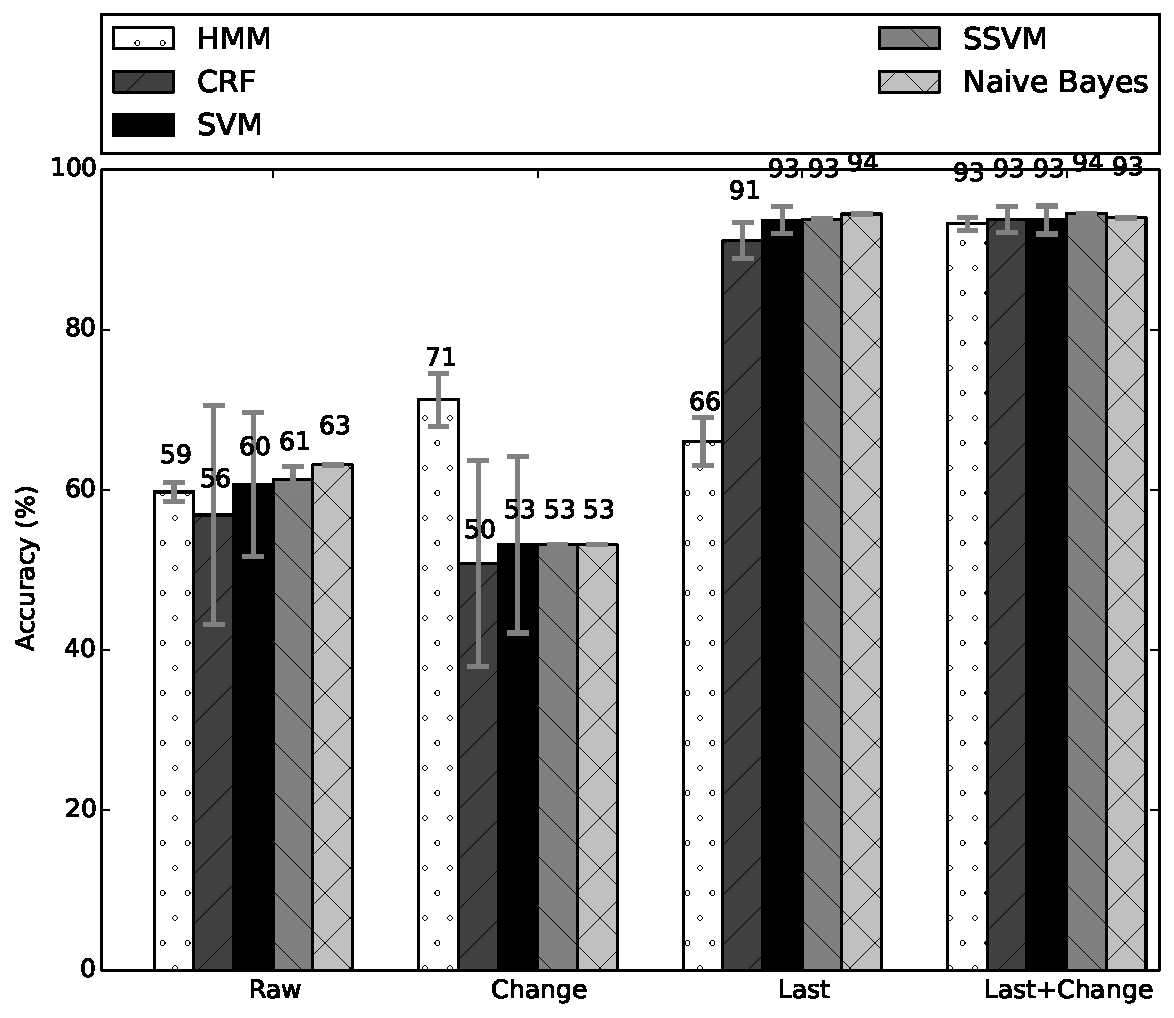
\includegraphics[width=5in]{../../src/reports/A.pdf}
%\end{center}
%\vspace{-0.5cm}
%\caption{House A}
%\label{fig:house_a}
%\vspace{-0.5cm}
%\end{figure}
%
%\begin{figure}[t!]
%\begin{center}
%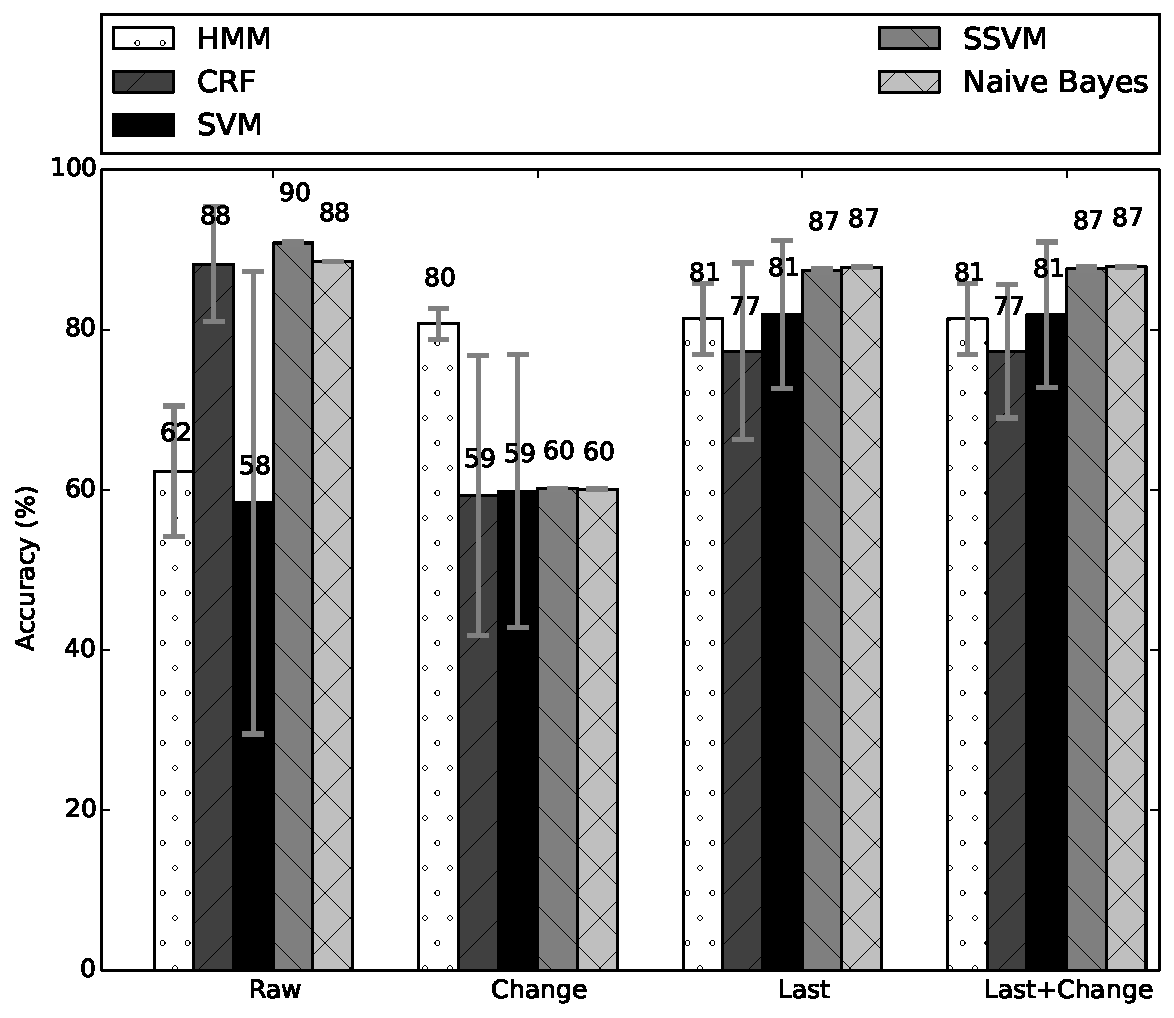
\includegraphics[width=5in]{../../src/reports/B.pdf}
%\end{center}
%\vspace{-0.5cm}
%\caption{House B}
%\label{fig:house_b}
%\vspace{-0.5cm}
%\end{figure}
%
%\begin{figure}[t!]
%\begin{center}
%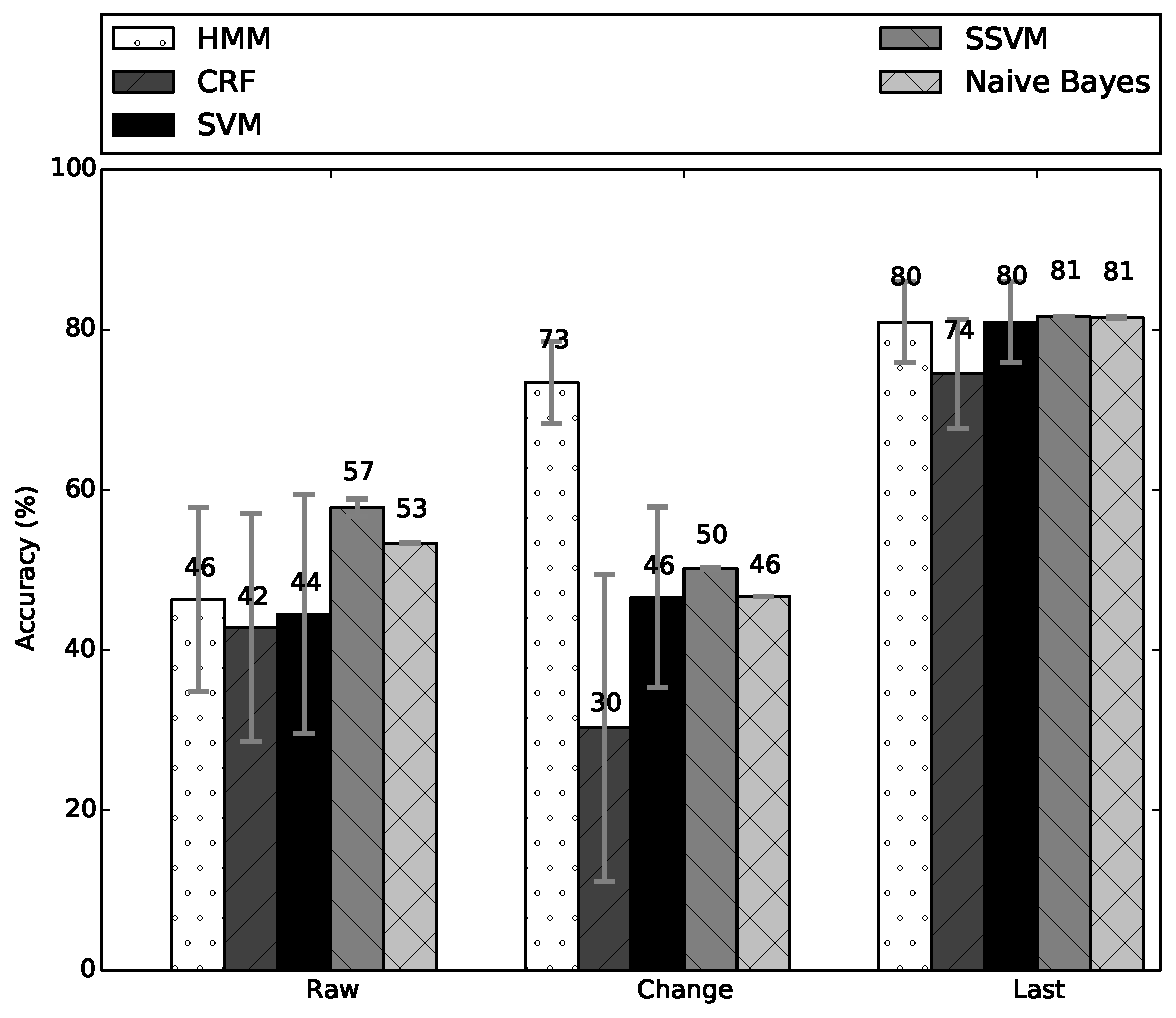
\includegraphics[width=5in]{../../src/reports/C.pdf}
%\end{center}
%\vspace{-0.5cm}
%\caption{House C}
%\label{fig:house_3}
%\vspace{-0.5cm}
%\end{figure}

